%%%%%%%%%%%%%%%%%%%%%%%%%%%%%%%%%%%%%%%%%%%%%%%%%%%%%%%%%%%%%%%%%%%%%%%%%%%%%%%%
\section{Unindo letra e música}
\label{sec:ProsodiaMusical}
\textbf{Prosódia musical} é a designação que se lhe dá ao procedimento de \cite[pp. 336]{medteoria}:
\begin{itemize}
\item ajustar as palavras à música, ou 
\item ajustar a música às palavras.
\end{itemize}

Para cumprir este objetivo, 
as sílabas tônicas das palavras devem coincidir com os acentos da música \cite[pp. 149]{medteoria} \cite[pp. 60]{howard1991aprendendo};
é importante lembrar que existem vários tipos de acentos na música,
como o \hyperref[def:acentometrico]{\textbf{acento métrico}}, 
o \hyperref[def:acentodinamico]{\textbf{acento dinâmico}}, etc.

~

Entre as decisões que devemos tomar quando queremos unir letra e melodia numa música, 
está a duvida de como dividir as palavras em relação as figuras musicais, pois podemos:
\begin{itemize}
\item Usar uma nota por silaba, 
o que provoca que a melodia imite a voz \cite[pp. 60]{howard1991aprendendo},
como quando se ouve a uma criança muito pequena falar.
\item Usar um conjunto de notas para cada sílaba, 
distanciando-nos da forma falada, dando-lhe um efeito musical à voz \cite[pp. 60]{howard1991aprendendo}. 
\end{itemize}
Ambos enfoques ao problema são válidos, 
na prática o compositor optará por trabalhar em algum ponto intermediário
entre estas duas abordagens \cite[pp. 60]{howard1991aprendendo}.


\PRLsep{Recomendações}

Existem algumas recomendações interessantes de ser tomadas em conta na hora de associar letra e melodia:
\begin{itemize}
\item As notas com maior \hyperref[sec:pos:Altura]{\textbf{altura}} precisam ser vinculadas a vogais abertas,
 que são mais fáceis de pronunciar \cite[pp. 61]{howard1991aprendendo}.
\item Devemos evitar coincidir os acentos da música com as sílabas átonas das palavras.
Se uma sílaba tônica de uma palavra já foi acentuada na música 
e se o comprimento da palavra nos restringe,
então é possível colocar uma acento numa sílaba átona da palavra. 
\item As palavras que são acentuadas na música devem ser palavras com significado \cite[pp. 61]{howard1991aprendendo},
como:
\begin{itemize}
\item substantivos (garrafa, rocha, amor, etc), 
\item adjetivos (linda, alegre, triste,etc), 
\item verbos (amar, sofrer, andar, etc), 
\item advérbios (nunca, melhor, ali, etc), 
\item pronomes (Eu, você, ele,algum,  nós, etc), 
\item numerais (duplo, quatro, oito,etc), 
\item interjeições (boa!, ah!!, ufa!, oxalá!, etc); 
\end{itemize}
em geral se acentuam as palavras que trazem informação.
\item Evitar acentuar palavras de ligação sem significado, como: 
\begin{itemize}
\item preposições e conjunções (de, por, em, e, mas, ou, etc),
\item pronomes relativos e artigos (me, se, te, que, o, a, etc).
\end{itemize}
\end{itemize}


\PRLsep{O propósito da letra na música}

Em geral o propósito de associar letra e melodia é ressaltar o significado das palavras;
pois se não fosse assim bastaria com deixar só a parte instrumental.
Assim, deve ser respeitada a acentuação das palavras na melodia para que estas não percam seu sentido;
porém, isto não quer dizer que as regras da língua devam ser respeitadas a toda costa; 
pois em muitas ocasiões o compositor deseja ressaltar na sua letra algum jeito diferente de falar ou regionalismo. 
Em geral, devemos chegar a um compromisso entre a forma de falar e 
a eficiência na transmissão da mensagem na letra da música.



\PRLsep{Exemplos}

\begin{example}[Encaixando uma frase na métrica:]
\label{ex:prosodia1}
A seguinte figura mostra uma frase de 5 palavras, indicando onde se encontra a sílaba tônica.
\begin{center}
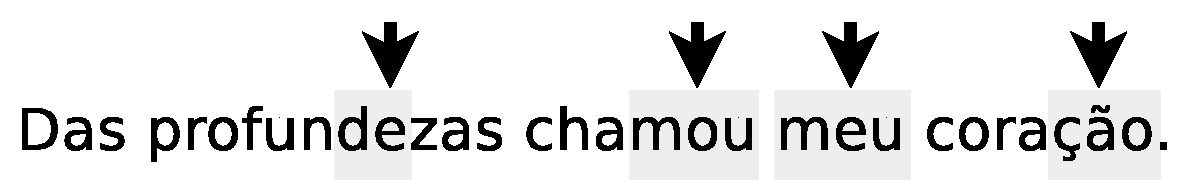
\includegraphics[width=0.65\textwidth]{chapters/cap-musica-topicos/prosodia1.eps}
\end{center}
Da frase anterior, os pontos mais interessantes são:
\begin{itemize}
\item ``meu'', que é um monossilabo tônico, pois é um pronome possessivo; e
\item ``das'', que é um monossilabo átono, pois é uma contração de preposição.
\end{itemize}
Esta frase pode ser ajustada na pauta usando a métrica dos compassos;
um possível resultado é o seguinte:
\begin{center}
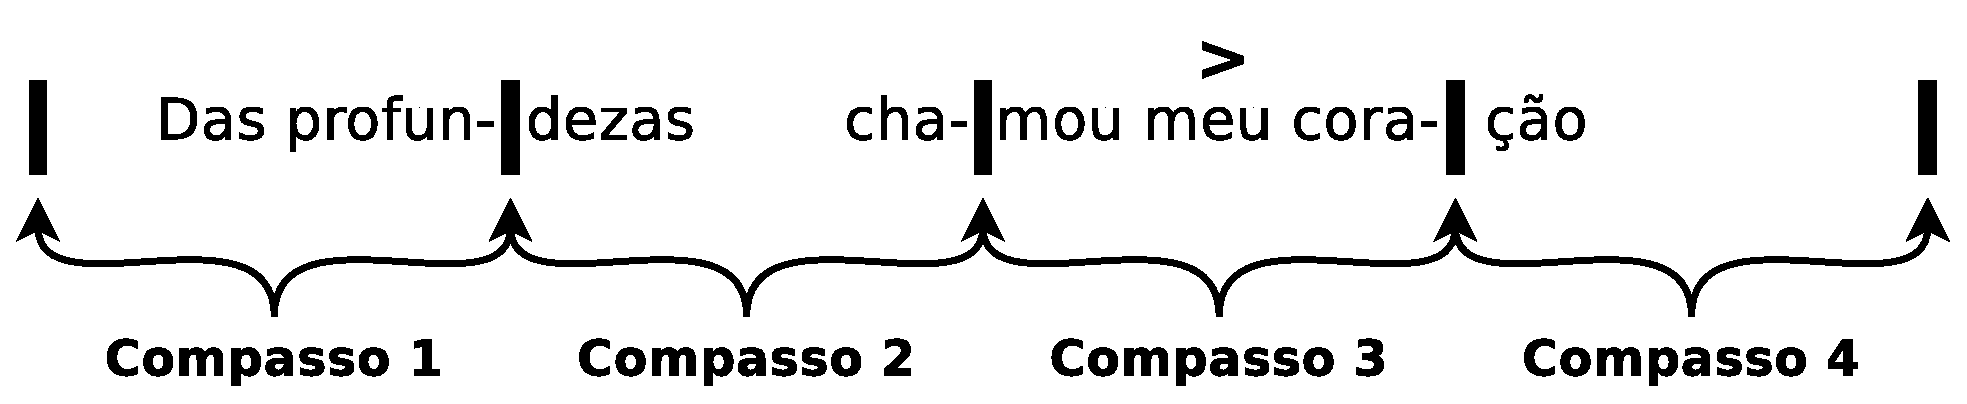
\includegraphics[width=0.95\textwidth]{chapters/cap-musica-topicos/prosodia2.eps}
\end{center}
É fácil ver que todas as sílabas tônicas foram corretamente 
aproveitadas pela métrica nos compassos,
porém em alguns casos as silabas foram ligeiramente alongadas, a comparação de uma fala natural,
para que a palavra seguinte encaixe na métrica.
Isto acontece de forma recorrente na música. 
\end{example}

%%%%%%%%%%%%%%%%%%%%%%%%%%%%%%%%%%%%%%%%%%%%%%%%%%%%%%%%%%%%%%%%%%%%%%%%%%%%%%%%
\begin{example}[Procurando o ritmo da frase:]
\label{ex:prosodia2}
Continuando o Exemplo \ref{ex:prosodia1}, podemos atribuir um ritmo à frase; 
neste exemplo foi escolhido usar uma nota por sílaba, 
procurando uma duração próxima à usada na fala natural.
Na seguinte figura vemos o ritmo obtido ao seguir o procedimento anteriormente explicado. 
\begin{center}
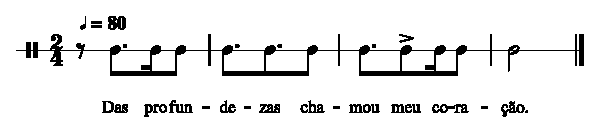
\includegraphics[width=0.95\textwidth]{chapters/cap-musica-topicos/frase5a-1.eps}
\end{center}
\end{example}

%%%%%%%%%%%%%%%%%%%%%%%%%%%%%%%%%%%%%%%%%%%%%%%%%%%%%%%%%%%%%%%%%%%%%%%%%%%%%%%%
\begin{example}[Desenhando a melodia de uma frase rítmica:]
\label{ex:prosodia3}
Finalmente, e concluindo o Exemplo \ref{ex:prosodia2}, 
para atribuir \hyperref[sec:pos:Altura]{\textbf{alturas}} (tons) a cada figura musical na frase rítmica, 
foi escolhido continuar imitando a fala\footnote{O 
critério na escolha de \hyperref[sec:pos:Altura]{\textbf{alturas}} pode ser visto na Pag. \pageref{ref:minhasvogais} (Minhas vogais).}
humana,
assim as alturas foram selecionadas guardando proporção com as alturas da fala numa conversa.
\begin{center}
\href{https://drive.google.com/file/d/1LshTD9MsnL2LU70VyLBLKnlghprm0x8P/view?usp=sharing}{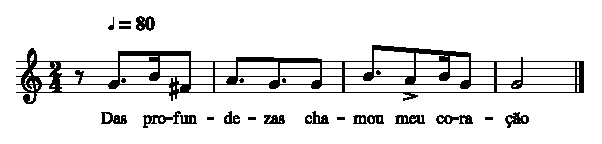
\includegraphics[width=0.95\textwidth]{chapters/cap-musica-topicos/frase5-1.eps}}
\end{center}
\end{example}

%%%%%%%%%%%%%%%%%%%%%%%%%%%%%%%%%%%%%%%%%%%%%%%%%%%%%%%%%%%%%%%%%%%%%%%%%%%%%%%%
\begin{figure}[!ht]
\begin{elaboracion}{Minhas vogais}
Foi realizado, na Pag. \pageref{fig:timbresvocais}, um analises da relação das frequências principais nas vogais,
durante uma fala natural (ex: uma conversa);
obtendo-se uma distribuição de alturas que não encaixava perfeitamente numa grade em semitons.
Porém, fazendo um pequeno esforço no controle da voz, 
é possível imaginar que é atingível a seguinte distribuição de alturas.
\begin{center}
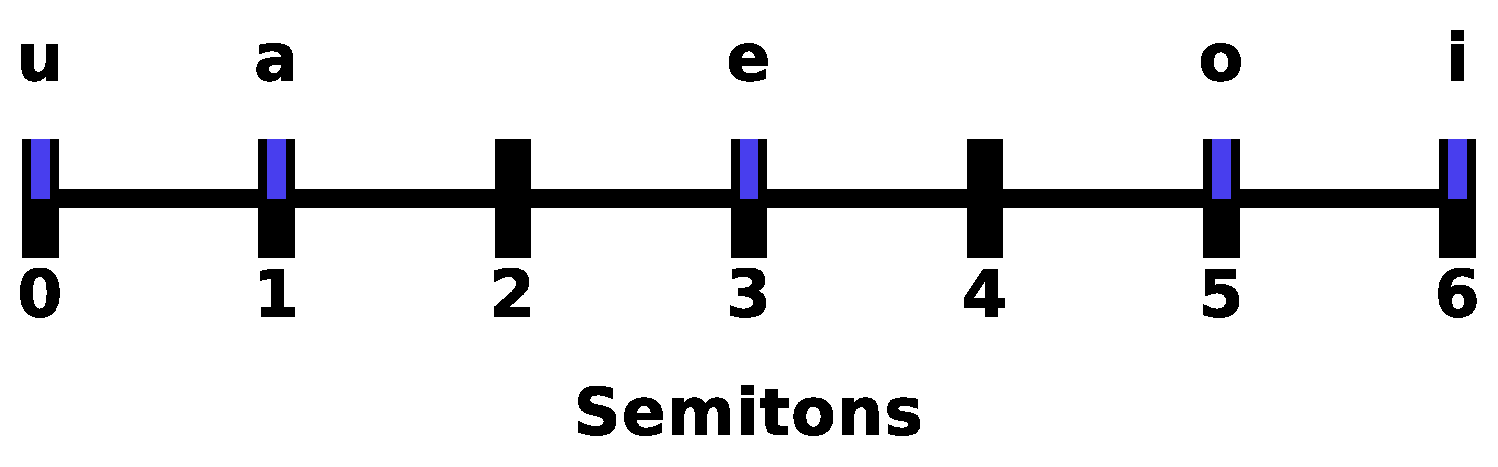
\includegraphics[width=0.50\textwidth]{chapters/cap-musica-topicos/vocales-semitons2.eps}
\end{center}
Assim, se nossa intenção numa composição musical é imitar a fala, 
então uma opção seria escolher notas musicais, 
com alturas numa proporção próxima às alturas das vogais na nossa fala, 
como a mostrada na figura anterior.
Estas proporções de alturas correspondem a uma forma particular de falar e não pode ser generalizada a outras pessoas;
de modo que, um cantor com um bom domínio da voz poderia atingir maiores rangos tonais.
Por exemplo, a revista peruana ``Caretas'' (2008)  menciona sobre a cantante ``Yma Sumac'',
que esta possuía uma rango vocal de 5 \hyperref[sec:pos:Oitava]{\textbf{oitavas}} \cite[pp. 73]{2008caretas}.  
\end{elaboracion}
\label{ref:minhasvogais}
\end{figure}




% https://es.wikipedia.org/wiki/Letra_(m%C3%BAsica)
% https://vox-technologies.com/blog/como-escribir-letras-de-canciones


